\chapter{Analysis and Modelling}
\label{chap:evaluation}

As outlined in the previous chapter, two sets of experiments were conducted to characterise a highly interactive video-on-demand system, as well as to test some new content management techniques. In this chapter, we use traces from our system to characterise user behaviour and the resulting workload. Using a combination of {\em R-Square} fitting and {\em Kolmogorov-Smirnov tests}, models for the various features were determined. Aggregated results are shown where applicable, but in some cases it is more appropriate to show results for individual videos. We noted in many cases that the features analysed were similar for each video, so for simplicity we will specifically discuss two individual videos in greater detail: the World Cup's Argentina \emph{vs.} Serbia and Montenegro match, and the Eurovision Song Contest final. Both were amongst the top~5 most popular videos and were representative of their genres (namely sport and music). We will refer to these files as \emph{arg-scg} and \emph{eurovision} respectively.

%We display results from both experiments, the 2006 FIFA World Cup and the later Eurovision. The Worldcup ran from the $9^{th}$ of June until the $9^{th}$ of July, however the results analysed in this paper were
%recorded from the $13^{th}$ of June until the $16^{th}$ of July. The
%data for the first 4 days was discarded due to alterations made to
%the logging system and user interface in that period. Also, the 7
%extra days considered after the end of the World Cup were added due
%to continued use of the site. The Eurovision experiment A total of 66 matches were logged (64
%from the event, and 2 pre-competition friendlies), with 405 unique
%users over the one month period. On average 30.7 unique users viewed
%each match.

Throughout the two experiments we observed a total of \verb+~+1800 unique users to the site, with each video receiving on average 68.2 unique users (and an overall maximum of 383). During this period we served 925 hours of video, which equates to 3.3~terabits of data. We received an average demand of 287$\pm$31 requests per day, with Thursday being the most popular. Throughout the day we saw the typical diurnal sinusoidal access patterns averaging 12$\pm$10 requests per hour, reaching its peak at midday with an average demand of 29 requests per hour.

We witnessed 123 unique users for \emph{arg-scg}, and 131 unique users for \emph{eurovision}, who watched for a combined total of 29.1~hours and 79.6~hours respectively. Note that if an individual does not maintain the same HTTP cookie between sessions (\emph{e.g.}, their cookie is deleted) they will appear as a new unique user. Equally, if two individuals share the same cookie, they will appear as a single unique user. While we expect these cases to be rare, they may however introduce error into the unique user count.

An observant reader will note that the most popular video had 383 unique users, yet the analysis is concentrated on \emph{arg-scg} and \emph{eurovision} with only 123-131 unique users. The reason for this is that the most popular content, a collection of `cheesy' music videos, had a very short average session duration. The video was the newest content on the site for many weeks, as such was at the top of the list of videos. We speculate that newcomers to the site would click on this video to understand what the site had to offer, but quickly stop. Shortly afterwards they would continue to explore the other videos on the site, which were perhaps better to their liking. These shorts views were therefore not representative of a typical viewing session and thus the analysis does not concentrate on them.

% What metrics we looked at, why? and what else?
The rest of this chapter uses the traces obtained from the experiments and characterises the observed user behaviour. Common metrics are looked at, such as popularity, longevity, session length, \emph{etc}. However, to describe the more interactive aspects, new analysis techniques and metrics were developed such as seek distance, hotspot length, jump plots and sequence graphs.

\section{Probability Distribution}

Throughout this chapter different metrics will be fitted to and modelled by different probability distribution. This section quickly outlines the main models, and discusses their uses and relevance.

\begin{description}
  \needspace{4\baselineskip}
  \item[Normal] {\Large $pdf(x;\mu,\sigma) = \frac{1}{\sigma \sqrt{2\pi}} \exp\left(-\frac{(x-\mu)^2}{2\sigma^2}\right)$ }

  A normal distribution is perhaps one of the simplest probability distribution also known as the Gaussian distribution, and recognised as the bell curve. Any variable which is the sum of multiple independent identically-distributed factors is likely to be normally distributed. This ensures that values are centered around a mean with a equal variance either side. There are many examples of normal distribution in natural, for example height of people or the intensity of laser light.
\end{description}

Other distribution are generally not centered around a mean and instead skewed. This is particularly common when mean values are low, variances large, and values cannot be negative~\cite{limpert2001lnd}. The follow distributions are all skewed.

\begin{description}
  \item[Log-normal] {\Large $pdf(x;\mu,\sigma) = \frac{1}{x \sigma \sqrt{2 \pi}}e^{-\frac{(\ln (x) - \mu)^2}{2\sigma^2}}$}

  Log-normal is a continuous distribution in which the logarithm of the variable is normally distributed. For example, if $X$ is a random variable with a normal distribution then $Y=e^X$ is a log-normally distributed. This distribution is generated by multiple independent variables in a similar way to a Normal distribution however, the variables are multiplied instead of added. Within video-on-demand analysis log-normal can be used to model the size of frames within a video stream, or in some cases the popularity of content~\cite{cha2007tyt}.

%  There are many uses of log-normal, but typically used when

  \item[Exponential] {\Large $pdf(x;\lambda) = \lambda e^{-\lambda x}$}

  Exponential is a simple continuous distribution which models the wait times between events, if events occur continuously and independently at a rate of $\lambda$ per unit of time. Typically it is used to measure the time between particle decays in radioactive materials, or the time between phone calls. More specifically it can model the time between viewing of a video.

  \item[Weibull] {\Large $pdf(x;\lambda,k) = \frac{k}{\lambda}\left(\frac{x}{\lambda}\right)^{k-1}e^{-(x/\lambda)^{k}}$}

  This is a particular flexible continuous probability distribution which can mimic the behavior of other statistical distributions such as the normal and the exponential. For example, when $k=1$ the distribution is identical to an exponential distribution, and when $k=3.4$ it resembles a Normal distribution. Weibull distributions are commonly used in survival analysis, reliability engineering and failure analysis, amongst others. In VoD it has been used to model the session times, as well as metrics more commonly used by an exponential distributions.

  \item[Poisson] {\Large $pmf(k; \lambda) = \frac{\lambda^k e^{-\lambda}}{k!}$}

  is a discrete distribution which expresses the probability that a number of events will occur in a fixed period of time when events occur independently of each other at a known average rate. This is typically used to model arrival distributions in multimedia systems such as the number of times a video is accessed in a particular period.

\end{description}

The following distribution are considered power law distributions. These are ones where the frequency of an event is proportional to its rank, \emph{i.e.} the $i$\sth most popular object receives $1/i^\alpha$ of requests.

\begin{description}
  \item[Pareto] {\Large $pdf(x;k) = \frac{k\,x_\mathrm{m}^k}{x^{k+1}}$}

  is a continuous power law probability distribution more simply known as the Pareto principle or the ``80-20 rule''. It states that 80\% of the distribution's weight is from only 20\% of the values. This has been observed in many examples, such as, the distribution of wealth or the distribution of file size in TCP transfer over the internet, \emph{etc}.

  \item[Zipf] {\Large $pmf(k; s,N) = \frac{1/k^s}{H_{N,s}}$}

  Zipfian distributions have become very popular in computer science, and may be thought of as a discrete counterpart of the Pareto distribution. It is used to model distributions where there are many large rare events, and many small common events. For example, the popularity of websites can be modelled by Zipf as there are millions of websites, which receive only a few users a day; and then there are a few large very popular websites. Zipf has also be shown to model the size of cities (there are a few mega-cities, but many small town) or used to model the frequencies that words occur, \emph{e.g.} words such as `and' and `the' that occur very frequently, but many which occur rarely.
\end{description}

\subsection{Fitting}

Throughout this Chapter the different evaluated metrics will be fitted to different mathematical models. There are a couple reasons to do this. Firstly, by fitting the raw data to a model it can aid in understand the shape and implications of the data. Secondly, by creating models it allows the models to be used for future simulations and experiments where using the raw data alone would not be suitable. Both of these reasons aids in the design and development of new algorithms and techniques, some of which are described in \autoref{chap:new_techiques}.

To test how good a models fits to the raw data two statistical tests were employed.

\begin{description}
  \item[R-square $R^2$]

    The R-Square is a very simple and common indicator of goodness of fit. It works by calculating the sum of the errors between the observed value and the value predicted by the model. More clearly it is defined as:
    \begin{equation}
        R^{2} = \frac{SS_{R}}{SS_{T}} = 1 - \frac{SS_{E}}{SS_{T}}
    \end{equation}

    where $SS_{R}$, $SS_{T}$ and $SS_{E}$ are defined as:
    \begin{equation}
        SS_{R} = \sum_{i=1}^n (\hat{y}_{i} - \bar{y})^{2}, ~~~
        SS_{T} = \sum_{i=1}^n (y_{i} - \bar{y})^{2}, ~~~
        SS_{E} = \sum_{i=1}^n (y_{i} - \hat{y}_{i})^{2}
    \end{equation}

    and the variables are defined as:
    \begin{itemize}
      \item $y_{i}$ is the observed value at $x_{i}$
      \item $\hat{y}_{i}$ is the value given by the model at $x_{i}$
      \item $\bar{y}$ is the mean value of $y_{1}...y_{n}$
      \item $n$ is the number of values.
    \end{itemize}

    The calculated $R^2$ value should be between $0$ and $1$, indicating how good a fit the model is to the real data, where 1 is a perfect fit, and 0 is a terrible fit.

  \item[Kolmogorov-Smirnov (K-S tests)]

    The Kolmogorov-Smirnov takes a different approach, instead it compares the empirical distribution function
(ECDF) of the data with the cumulative distribution function (CDF) of the model and simply measuring the largest distance between the two functions. The smaller the value the better the fit.
    \begin{equation}
        D = max_{i=1...n} ( CDF(y_{i}) - ECDF(y_{i}) )
    \end{equation}
\end{description}
By using a combination of $R^2$ and K-S tests it is possible to mathematically decide how well a parameterized model fits the real data. The remainder of the chapter will utilise these techniques to explain how well the models fit, and why they are suited to each particular metric.

\section{Interactions}
\label{sect:interactions}

%COMMENT
% AB: It was suggested that we justify why there is only one table or results, and it's not broken down per video/genre. I could find no statistical proof that the videos followed similar patterns. However this section is describing how our system in general experience lots of interactivity. As such I think a single aggregate table is fine.

Recall that our system allowed various interactive operations, namely pausing, resuming, seeking forwards \& backwards, and jumping to bookmarks. This range of operations, combined with the nature of the content, highly influenced user behaviour. As a result, for most users we observed a complete departure from the typical start-to-finish playback model that has been noted in previous work~\cite{costa2004aci}.

%TODO: Find a different reference than Costa04Analyzing, since we use Costa04Analyzing again 2 paragraphs later

\begin{table}[t]
\centering {\footnotesize
\begin{tabular}{|cccc|}
  \hline
\setrowcolor{TableRowHead}
  Action & Frequency & Percentage (\%) & Mean \& Std. ($\sigma$) per Session\\
  \hline
\setrowcolor{TableRowA}
  Back 10s        & 3098 & 4.50 & 0.59 ($\sigma=3.14$)\\
\setrowcolor{TableRowB}
  Back 30s        & 654  & 0.95 & 0.12 ($\sigma=0.83$)\\
\setrowcolor{TableRowA}
  Back 60s        & 1532 & 2.22 & 0.29 ($\sigma=1.90$)\\
\setrowcolor{TableRowB}
  Forward 10s     & 7438 & 10.79 & 1.41 ($\sigma=8.61$)\\
\setrowcolor{TableRowA}
  Forward 30s     & 1804 & 2.62 & 0.34 ($\sigma=2.93$)\\
\setrowcolor{TableRowB}
  Forward 60s     & 7930 & 11.51 & 1.50 ($\sigma=7.38$)\\
\setrowcolor{TableRowA}
  Seek-bar        & 9902 & 14.37 & 1.88 ($\sigma=7.39$)\\
\setrowcolor{TableRowB}
  Bookmarks       & 13857 & 20.11 & 2.62 ($\sigma=2.63$)\\
\setrowcolor{TableRowA}
  User bookmarks  & 1236  & 1.79 & 0.23 ($\sigma=1.01$)\\
%  Add bookmark    & ?   & & \\
\setrowcolor{TableRowB}
  Pause           & 11839 & 17.18 & 2.24 ($\sigma=7.65$)\\
\setrowcolor{TableRowA}
  Resume          & 9616 & 13.96 & 1.82 ($\sigma=6.80$)\\
% Restarts & 6920 & & \\

% 6920 sessions
% Bookmarks (ours): 459,  used 11 times on avg
% Bookmarks (theirs) 43, used 13.6 times on avg

  \hline
\end{tabular}
} \caption{Interactions observed throughout the experiment}
\label{tab:number_of_actions}
\end{table}

\autoref{tab:number_of_actions} shows, over the duration of the experiment, the frequency of each action and its corresponding percentage against all other operations. Small individual forward seeks were used a combined 24.9\% of the time, whereas individual backward seeking was only used 7.67\%. These actions only accounted for the short-seeks buttons (10, 30, and 60 seconds), whereas potentially large seeks (seek-bar and following bookmarks) made up 34.5\% of all operations. The table also shows that in each session (a viewing of a single video), a user on average used backward actions once, bookmarks and seek bar actions 4.5 times, and forward actions 3.25 times.

Previous studies have shown that the most common action is pause/resume~\cite{costa2004aci}, however we see that for our traces, forward operations are by far the most common, closely followed by seeking to bookmarks. The table also shows that the number of pause operations account for 17.18\% of all actions. Pausing not being the most common action can be explained by the short session durations observed. This is in accordance with previous work which found a positive correlation between session time and the number of pause operations~\cite{vilas2005uba}.

\begin{figure}[t]
    \centering

    %plotted with PlotJumps()
    \subfloat[][Argentina \emph{vs.} Serbia and Montenegro]{
        \label{fig:argscg_jumps}
        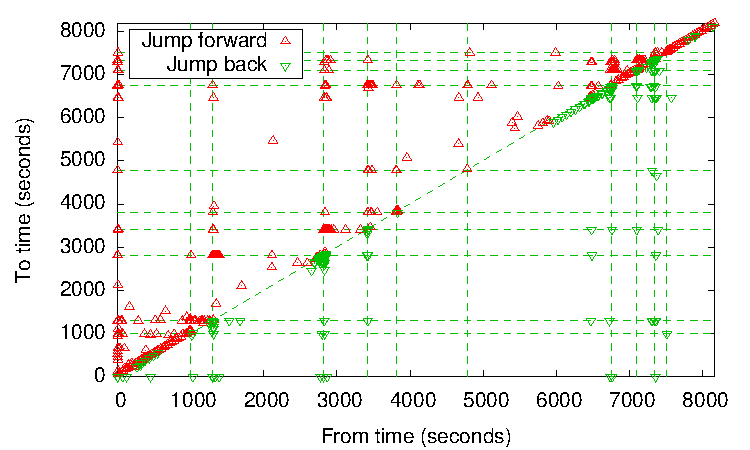
\includegraphics[width=0.5\columnwidth]{./graphs/arg-scg_jumps}
    }
    \subfloat[][Eurovision (cropped at 4000 seconds for clarity)] {
        \label{fig:eurovision_jumps}
        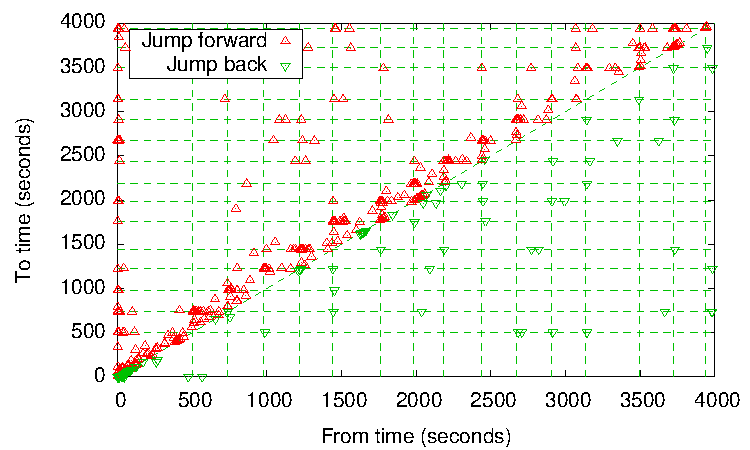
\includegraphics[width=0.5\columnwidth]{./graphs/eurovision_jumps}
    }

    \caption{Jumps made by users within two videos}
    \label{fig:jumps}
\end{figure}

To better understand how users navigated through a bookmarked video, we analysed the behaviour in the \emph{arg-scg} and \emph{eurovision} videos, which had 10 and 24 bookmarks respectively. In \autoref{fig:argscg_jumps} \& \autoref{fig:eurovision_jumps} each point is a seek that is identified by a ``from'' time on the x-axis and a ``to'' time on the y-axis. A point $x$,$y$ therefore represents a user that has jumped from their current playback point $x$ to a new point, $y$. Vertical and horizontal lines in the figures denote the position of the bookmarks. The diagonal line is a current-time marker such that seeks forward are points which lie above it, while seeks backward appear below it. Therefore, no point can fall precisely on the diagonal. It is immediately obvious from the figures that many points are on horizontal lines, implying that most seeks were to the bookmarks.

The forward seek buttons appear to have been mostly used for skipping to the next event, shown on both figures as points slightly above the diagonal line between the bookmarks. This could be due to user unfamiliarity with the bookmark interface, or possibly users simply browsing the video. Backward actions were typically used around bookmarks, where users would often re-watch the bookmarked event. In some cases users may also have wished to see video immediately preceding the bookmark. An example of this is shown in \autoref{fig:argscg_jumps} before the bookmark at time 2815, where users sought up to 75 seconds backwards to see more of the build up to the goal.

Clusters of points can also be seen on horizontal lines shortly after a vertical line, indicating that users jumped from bookmark to bookmark. In fact, the concentration of clusters of point just above the diagonal time reference indicates that users have a tendency to follow bookmarks in sequence, as exemplified in \autoref{fig:eurovision_jumps}.

Overall, for both videos these results demonstrate that users did not simply view continuously start-to-finish, and were in fact highly influenced when presented with bookmarks.

\section{Seek Distance}
\label{sect:seek_distance}

\begin{figure}[t]
    \centering

    \subfloat[][All seek distances] {
        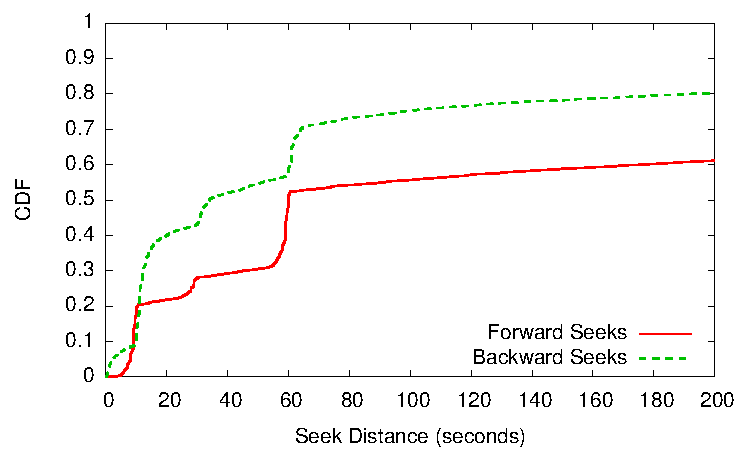
\includegraphics[width=0.5\columnwidth]{./graphs/all_jump_distance_200}
        \label{fig:seek_distance-a}
    }
    \subfloat[][All seeks cropped at 200 seconds] {
        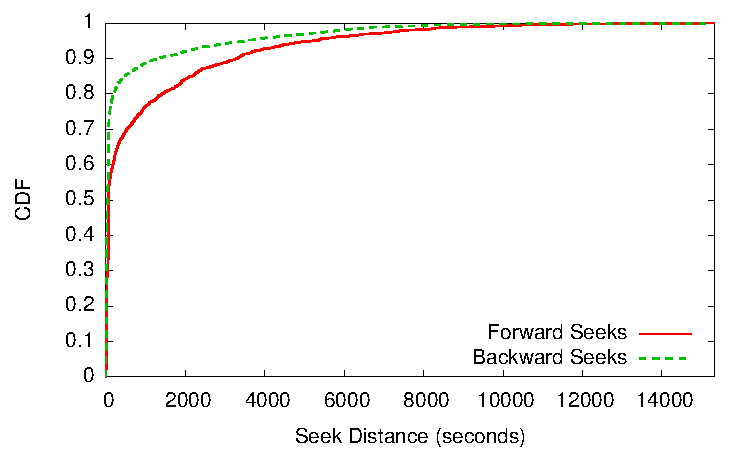
\includegraphics[width=0.5\columnwidth]{./graphs/all_jump_distance}
        \label{fig:seek_distance-b}
    }

    \caption{CDF of backward and forward seek distances}
    \label{fig:seek_distance}
\end{figure}

The understanding of locality is important for caching and pre-fetching algorithms. By looking at how far users sought we can determine the probability of accessing media nearby the playback point. We therefore define \emph{seek distance} as the absolute difference, in seconds, between a user's current playback point and their requested seek destination.

\autoref{fig:seek_distance-a} \& \autoref{fig:seek_distance-b} display a CDF of seek distance for backward and forward actions. A large proportion of seeks (between 50\%-70\%) are of a 15 seconds, 30 seconds, or 60 seconds values. These seeks represent the short seek button presses.
40\% of backward seeks were less than or equal to 15 seconds in length. This property could be exploited by keeping a small client side buffer of previously watched segments, which would satisfy many backward seeks if the user has already viewed them.
%The seeks do not occur exactly on their respective values because seeks can only be to a video keyframe, which were not always at exact second intervals.

% forwards mean 955.32
%  'Log-Normal'    'R_SQUARE ='    [0.96622]    'TEST ='    [58.528]    'MU ='[4.7599] 'SIGMA ='    [2.5265]
%  'Weibull'    'R_SQUARE ='    [0.94271]    'TEST ='    [96.206]    'l ='    [324.87] 'k ='    [0.42302]

% backwards mean 495.95
% 'Log-Normal'    'R_SQUARE ='    [0.96888]    'TEST ='    [21.927]    'MU ='    [3.6127] 'SIGMA ='    [1.7816]
% 'Weibull'    'R_SQUARE ='    [0.95186]    'TEST ='    [34.631]    'l ='    [69.156] 'k ='    [0.6563]

% forwards > 61 with mean 1968
% 'Log-Normal'    'R_SQUARE ='    [0.99259]    'TEST ='    [8.7149]    'MU ='    [6.8269] 'SIGMA ='    [1.5953]

% backwards > 61 with mean 1630
% 'Log-Normal'    'R_SQUARE ='    [0.98238]    'TEST ='    [4.5006]    'MU ='    [6.3273]  'SIGMA ='    [1.7906]

Even though small seeks are the majority, there are between 30\% and 50\% of seeks which are further than 60 seconds. These seeks consist of jumps to bookmarks or ``blind'' seeks with the seekbar. These long range seeks are log-normally distributed with a mean of 1968 seconds and 1630 seconds for forward and backward seeks respectively. They can be fitted to log-normal models with parameters $\mu = 6.8269$ and $\sigma = 1.5953$ for forward seeks, and $\mu = 6.3273$ and $\sigma = 1.7906$ for backward seeks. It can been seen that the backward distribution has a greater positive skew than the forward distribution, thus it will generate many small seeks.

%TODO add cool stat of how many of those 40\% rewinds could be satisified frmo a buffer

These behaviours exhibit a high degree of spatial locality, with the majority of seeks being within 60 seconds. Regarding long-ranged seeks, the log-normal distribution models imply that some very large distance seeks do occur, but the majority of seeks are shorter. Additionally, the skewed nature of this distribution is most likely because it is impossible to have a negative seek value. Overall the seek distances exhibit a median of 60 seconds for forward seeks and 34 seconds for backward seeks. This is consistent with previous findings~\cite{padhye1999cmc}.

%These behaviours exhibit a high degree of spatial locality, with the majority of seeks being within 60 seconds. Regarding long-ranged seeks, the log-normally distributed models imply that some very large distance seeks do occur, but the majority of seeks are shorter. Overall the seek distances exhibit a median of 60 seconds for forward seeks and 34 seconds for backward seeks. This is consistent with previous findings~\cite{padhye1999cmc}.

\section{Popularity}

\begin{figure}[t]
    % ploted with PlotPopularityRank()
    \centering
    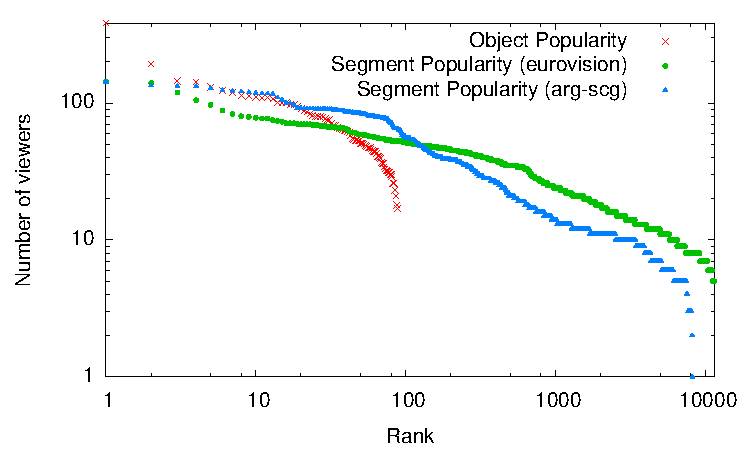
\includegraphics[width=0.5\columnwidth]{./graphs/all_sessions_rank}
    \caption{Object and segment popularity}
    \label{fig:popularity_object_rank}
\end{figure}

We study popularity in terms of the number of viewers who watched an \emph{object} or a \emph{segment}. An object in this system is a single video whereas a segment is a section of video one second in length.

The ranking for both object and segment popularity is shown in \autoref{fig:popularity_object_rank}. The \emph{eurovision}, and \emph{arg-scg} were approximately 10,000 seconds in length, causing \verb+~+10,000 segments to be ranked for each video. Recall that only 88 videos were available, so the lowest object rank is 88.

Typically object popularity with CDNs and VoD systems follows a power-law distribution~\cite{chesire2001maa,almeida2001aem,yu2006uub}, however, our analysis reveals otherwise. Instead the ranking of objects best fitted a normal distribution with parameters $\mu = 60$ and $\sigma = 32$. There are two reasons that power-law was not the best fit. Firstly, the catalogue of 88 videos was not very large, and secondly, power-law distributions do not fit well if the objects are constantly changing. Instead power-law fits better if a snapshot of rank \emph{vs.} popularity is taken each day and aggregated.

%Our analysis reveals that object popularity does not follow the typical power-law distribution observed within CDNs~\cite{chesire2001maa,almeida2001aem,yu2006uub} but instead is a normal distribution with parameters $\mu = 60$ and $\sigma = 32$. This can be attributed to the nature of our videos and the relatively few new objects each day.

% object pop (using rsqare)
%'Log-Normal'    'R_SQUARE ='    [0.99735]    'TEST ='    [0.015259]    'MU ='    [4.0391]    'SIGMA ='[0.55552]
%'Normal'    'R_SQUARE ='    [0.97996]    'TEST ='    [0.11636]    'MU ='    [60.129]    'SIGMA ='    [32.111]
%'Weibull'    'R_SQUARE ='    [0.99116]    'TEST ='    [0.050083]    'l ='    [70.549]    'k ='    [2.0227]

% object pop (using kst)
%'Log-Normal'    'R_SQUARE ='    [0.99708]    'TEST ='    [0.03116]    'MU ='    [4.03]    'SIGMA ='[0.55872]
% 'Normal'    'R_SQUARE ='    [0.97993]    'TEST ='    [0.077785]    'MU ='    [59.79]    'SIGMA ='    [30.131]
%'Weibull'    'R_SQUARE ='    [0.99039]    'TEST ='    [0.05571]    'l ='    [69.301]    'k ='    [2.114]


\begin{figure}[t]
    \centering

    %plotted with PlotViews()

    \subfloat[][Argentina vs. Serbia and Montenegro] {
        \label{fig:arg-scg_views}
        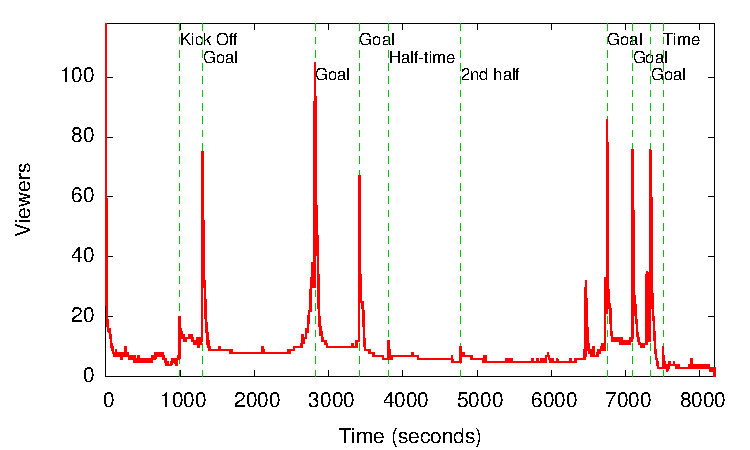
\includegraphics[width=0.5\columnwidth]{./graphs/arg-scg_views}
    }
    \subfloat[][Eurovision] {
        \label{fig:eurovision_views}
        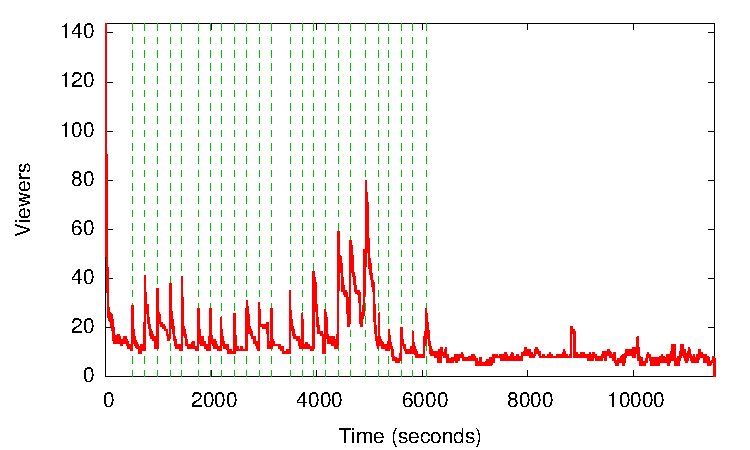
\includegraphics[width=0.5\columnwidth]{./graphs/eurovision_views}
    }

    \caption{Number of viewers at each second of video (each vertical line represents the position of a bookmark)}
\end{figure}

% euro (using rsquare)
%'Log-Normal'    'R_SQUARE ='    [0.99254]    'TEST ='    [0.035621]    'MU ='    [2.3233]    'SIGMA =' [0.56684]
%'Poisson'    'R_SQUARE ='    [0.95483]    'TEST ='    [0.24824]    'l ='    [11.142]
%'Weibull'    'R_SQUARE ='    [0.97982]    'TEST ='    [0.095445]    'l ='    [12.782]    'k ='    [1.8621]


% euro (using kst)
%'Log-Normal'    'R_SQUARE ='    [0.98993]    'TEST ='    [0.047187]    'MU ='    [2.3188]    'SIGMA ='    [0.49565]
%'Poisson'    'R_SQUARE ='    [0.95477]    'TEST ='    [0.14129]    'l ='    [11.132]
%'Weibull'    'R_SQUARE ='    [0.97678]    'TEST ='    [0.076196]    'l ='    [12.709]    'k ='    [2.3226]

% arg-scg (using rsqare)
%'Log-Normal'    'R_SQUARE ='    [0.99463]    'TEST ='    [0.03468]    'MU ='    [2.0063]    'SIGMA ='[0.58707]
%'Poisson'    'R_SQUARE ='    [0.98022]    'TEST ='    [0.13836]    'l ='    [8.5039]
% 'Weibull'    'R_SQUARE ='    [0.98978]    'TEST ='    [0.065082]    'l ='    [9.3509]    'k ='    [1.9405]

% arg-scg (using kst)
%'Log-Normal'    'R_SQUARE ='    [0.99428]    'TEST ='    [0.043658]    'MU ='    [2.0248]    'SIGMA ='[0.54523]
%'Poisson'    'R_SQUARE ='    [0.97926]    'TEST ='    [0.099252]    'l ='    [8.2927]
%'Weibull'    'R_SQUARE ='    [0.98943]    'TEST ='    [0.059218]    'l ='    [9.3725]    'k ='    [2.1449]

% all (using rsquare)
%'Weibull'    'R_SQUARE ='    [0.98284]    'TEST ='    [0.048803]    'l ='    [2.887]    'k ='    [0.69527]
%'Log-Normal'    'R_SQUARE ='    [0.98084]    'TEST ='    [0.054389]    'MU ='    [0.55114]    'SIGMA =' [1.3233]
%'Normal'    'R_SQUARE ='    [0.95011]    'TEST ='    [0.11357]    'MU ='    [2.5469]    'SIGMA ='    [3.4551]
%'Pareto'    'R_SQUARE ='    [0.94499]    'TEST ='    [0.13353]    'k ='    [0.97715]
%'Poisson'    'R_SQUARE ='    [0.92442]    'TEST ='    [0.2116]    'l ='    [2.923]
%'Zipf'    'R_SQUARE ='    [0.92855]    'TEST ='    [0.16903]    's ='    [1.7921]


% all (using kst)
%'Log-Normal'    'R_SQUARE ='    [0.965]    'TEST ='    [0.21597]    'MU ='    [0.95]    'SIGMA ='    [1.05]
%'Pareto'    'R_SQUARE ='    [0.94402]    'TEST ='    [0.21597]    'k ='    [1]
%'Normal'    'R_SQUARE ='    [0.93512]    'TEST ='    [0.13497]    'MU ='    [2.3933]    'SIGMA ='    [2.1693]
%'Zipf'    'R_SQUARE ='    [0.92861]    'TEST ='    [0.21597]    's ='    [1.79]
%'Poisson'    'R_SQUARE ='    [0.92163]    'TEST ='    [0.16872]    'l ='    [2.8265]

% Some matlab code to work out the top X %
% a = all_views(:,2);
% [y, x] = ecdf(a);
% x ( find(y > 0.99) ); limit = ans(1)
% sum( a ( find ( a > limit ) ) ) / sum( a )

% top 1% = 12% of requests
% top 10% = 44% of requests

%The popularity of one-second segments for all the videos exhibit a Weibull distribution with parameters $\lambda=2.887$
Again, the popularity of one-second segments might be best suited by a power-law, however Zipf and Pareto did not fit well. Instead, the popularity of one-second segments for all the videos exhibit a Weibull distribution with parameters $\lambda=2.887$ and $k=0.69527$. Log-normal distributions provide the best fits for the  \emph{arg-scg} and \emph{eurovision} results independently with parameters $\mu = 2.00, \sigma = 0.587$ and $\mu = 2.32, \sigma = 0.567$ respectively. Note that log-normal and Weibull distributions closely relate to power-law or heavy-tailed distributions~\cite{mitzenmacher2004abh,fishman2006hht}: they are skewed distributions where a small percentage of samples contributes to a sizeable weight of their distribution. We observe that a small percentage, (the 10\% most popular segments), accounted for about 44\% of all requests. Previously, Costa~\emph{et~al.}~\cite{costa2004aci} found that for educational and entertainment content, the popularity of segments is roughly uniformly distributed with a slight skew towards the beginning for entertainment content. Our result, however, implies that there are segments with orders of magnitude more viewers than others.

To illustrate the order-of-magnitude differences in viewers, we present \autoref{fig:arg-scg_views} \& \autoref{fig:eurovision_views} which show the popularity of each second of video for \emph{arg-scg} and \emph{eurovision} respectively. The vertical lines signify the position of the bookmarks; note for the \emph{eurovision} video there were no bookmarks after 6000 seconds as only the performances were bookmarked and they all appeared in the first half of the video. It is clear from the figures that there are peaks of popularity, highly influenced by the bookmarks. In \emph{arg-scg} (and in other sport content) we observe that most of the bookmarks are equally popular. However, in the \emph{eurovision} (and other music genres), we observe there is a greater variance in the popularity of the bookmarks. This can be attributed to sports having numerous events which all users wish to watch, however in music videos there may be only certain artists which interest the user.

Popularity metrics are important to many CDN algorithms as they help to decide which resources to allocate to each object. We have seen that bookmarks within videos cause segments to be of high interest and popularity, for example, goals within a sporting event. This result emphasises the use of partial caching techniques~\cite{chen2003aal} to cache only popular segments.

\section{Longevity}
\label{sect:stay_popular}

\begin{figure}[t]
    % plotted with PlotPopularityLifetime()
    \centering
    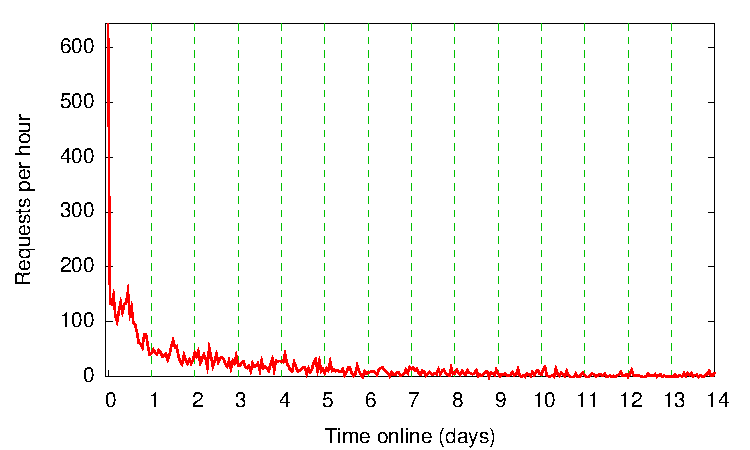
\includegraphics[width=0.5\columnwidth]{./graphs/all_bookpop_lifetime}
    \caption{Bookmark utilisation within all videos over time, following initial usage}
    \label{fig:lifetimes}
\end{figure}

%    'Weibull'    'R_SQUARE ='    [0.99796]    'TEST ='    [0.042635]    'l ='    [3.1004]    'k ='    [0.61592]
%    'Log-Normal'    'R_SQUARE ='    [0.98626]    'TEST ='    [0.28989]    'MU ='    [0.52115]    'SIGMA ='    [1.5475]

The popularity of both videos and bookmarks in our system changed over time. This phenomenon is outlined in \autoref{sect:pop_over_time} which describes how and why the popularity changes. However, in our results the popularity always declined, therefore we call the duration at which any such item remains utilised its \emph{longevity}. The study of a video or bookmark's longevity can aid cache replacement policies, as well as other content management decisions.

\autoref{fig:lifetimes} shows the popularity of all our bookmarks versus the time they were first used. The figure suggests that following an initial peak and a slight resurgence, there was a rapid decrease in interest after a short period. R-Square fitting reveals that the bookmark longevity can be suitably estimated using a Weibull distribution with $\lambda=3.10$ and $k=0.615$. This suggests that the popularity exhibits long-tailed properties. We also observe that 40\% of the bookmark usage occurs within 24 hours, with the remainder slowly occurring over the following weeks. This is in line with the previous research on this topic~\cite{cherkasova2004aoe}.

The popularity of videos decreased over time, but this is not true for the popularity of segments within the videos. For example, the segments which were popular within that video when it was first published were still popular within the video weeks later, long after the video had lost it overall popularity. This was tested on each video by calculating the distribution of segment popularity for the first 50\% of requests versus the last 50\% of requests. The difference in distributions was minor, with an average R-Square value of 0.9. On a visual inspection of the number of viewers per second, it was clear that the popularity still focused around the bookmarks.

\section{Session Lengths}

\begin{figure}[t]
    \centering
    %plotted with PlotSessions()

%    \subfigure[All videos] {
%        \label{fig:view_user_session}
%        \includegraphics[width=0.5\textwidth]{./graphs/all_user_sessions}
%    }
    \subfloat[][Eurovision] {
        \label{fig:eurovision_user_session}
        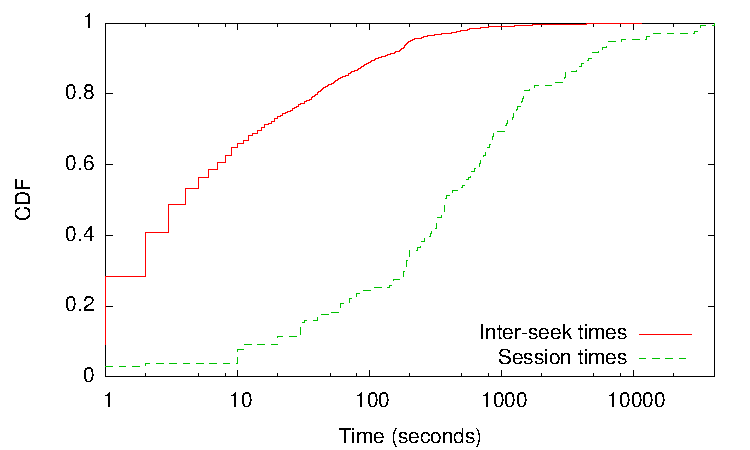
\includegraphics[width=0.5\columnwidth]{./graphs/eurovision_user_sessions}
    }
    \subfloat[][Argentina vs. Serbia and Montenegro] {
        \label{fig:arg-scg_user_sessions}
        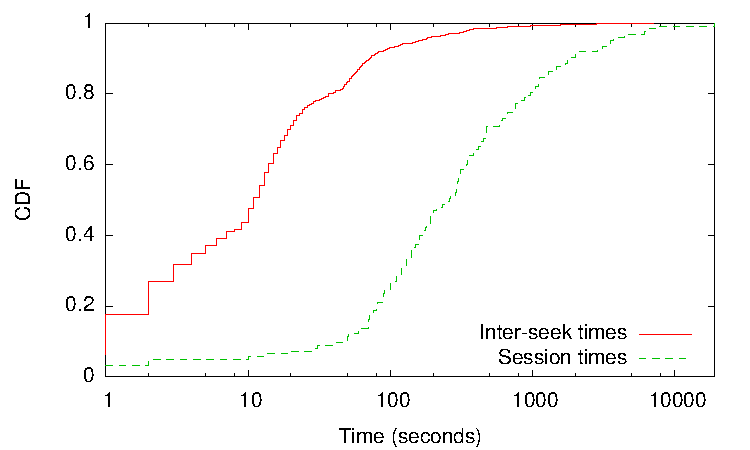
\includegraphics[width=0.5\columnwidth]{./graphs/arg-scg_user_sessions}
    }

    \caption{CDFs of session lengths and inter-seek times}
    \label{fig:view_user_sessions}
\end{figure}

Session length is the total time a user accessed a video, regardless of the actions they may have taken whilst doing so. For example, a session may be longer than the actual length of the video if the user chose to re-watch segments, and/or pause.

\autoref{fig:eurovision_user_session} \& \autoref{fig:arg-scg_user_sessions} show the CDF of both session and inter-seek times (discussion of inter-seek times follows in the next subsection). It can be observed from the session times that most users access each video for a very short time relative to its overall length (possibly just watching the events they are interested in). In particular, note that in the \emph{arg-scg} case around 80\% of sessions lasted less than 15 minutes. Given that the video was 2.2 hours in length, 15 minutes corresponds to only 11\% of the total video. A similar result was found with \emph{eurovision}, with 80\% of sessions lasting less than 12\% of the total video duration. The average session duration was found to be only 11 minutes and 18 minutes for \emph{arg-scg} and \emph{eurovision} respectively.

We also found that a small minority (roughly 3\%) of session durations were longer than the length of a video. Of these durations roughly 39\% were between 3 to 8 hours long. Our logs show that these users paused for a long time before deciding to resume playback.

%These outliers are possibly why we observe that session sizes are best fitted by a log-normal distribution with parameters $\mu=4.73$ and $\sigma=1.90$.

%    'Log-Normal'    'R_SQUARE ='    [0.99779]    'TEST ='    [0.1091]    'MU ='    [4.7315]    'SIGMA ='[1.9014]
%    'Normal'    'R_SQUARE ='    [0.86057]    'TEST ='    [7.3338]    'MU ='    [143.77]    'SIGMA ='    [489.46]
%    'Weibull'    'R_SQUARE ='    [0.98666]    'TEST ='    [0.65005]    'l ='    [233.17]    'k ='    [0.51125]

\section{Inter-seek Times}
\label{sect:interseek}

Inter-seek time is described as the duration for which a user watched a section of a video before seeking to a new location (disregarding any paused periods). This can be useful, for example, to determine the amount to replicate when using partial caching.

From our logs, we found that on average a user performed 8.98 seek operations around a video, resulting in a mean inter-seek time of 50.4 seconds. \autoref{fig:eurovision_user_session} \& \autoref{fig:arg-scg_user_sessions} show the CDF for inter-seek times as well as session length. As the inter-seek times are generally shorter than session times, this implies that the majority of users viewed the content as a series of excerpts, usually under a minute in length.

%It can been seen that around 50\% of viewed sections of videos were
%less than 8 seconds in length, and around 80\% of users watched the
%video for less than 50 seconds before seeking again. Less than 1\%
%of all users watched more than 1000 seconds of consecutive video.


%'Log-Normal'    'R_SQUARE ='    [0.99644]    'TEST ='    [0.020535]    'MU ='    [1.2886]    'SIGMA ='    [2.318]
%'Zipf'    'R_SQUARE ='    [0.91125]    'TEST ='    [0.36561]    's ='    [1.483]
%'Pareto'    'R_SQUARE ='    [0.92868]    'TEST ='    [0.30414]    'k ='    [0.57246]
%'Weibull'    'R_SQUARE ='    [0.99353]    'TEST ='    [0.037535]    'l ='    [7.5243]    'k ='    [0.35646]


The inter-seek time in the music content was found to be on average longer. This is because the length of a bookmarked musical performance generally exceeds the length of an event within a football match. Regardless of the difference in inter-seek times, we found that they can be estimated by log-normal distributions. For instance, the inter-seek time for \emph{arg-scg} can be modelled with parameters $\mu=2.15$ and $\sigma=1.72$.

Previous studies have found that the majority of inter-seek times are very short~\cite{vilas2005uba}. For long educational content, inter-seek times have also been shown to be Weibull distributed or a combination of Weibull for
the body and Pareto for the tail~\cite{almeida2001aem}. We found that most of our videos had inter-seek times that could be suitably modelled by a Weibull distribution, and two thirds which could be modelled with Pareto alone. Models of inter-seek times can be used by a delivery system to determine the size of video replicas and the time available to react before a user seeks elsewhere in the video.

\section{Sequence}
\label{sect:sequence}

% TODO Place both figures next to each other
\begin{figure}[t]
    \centering
    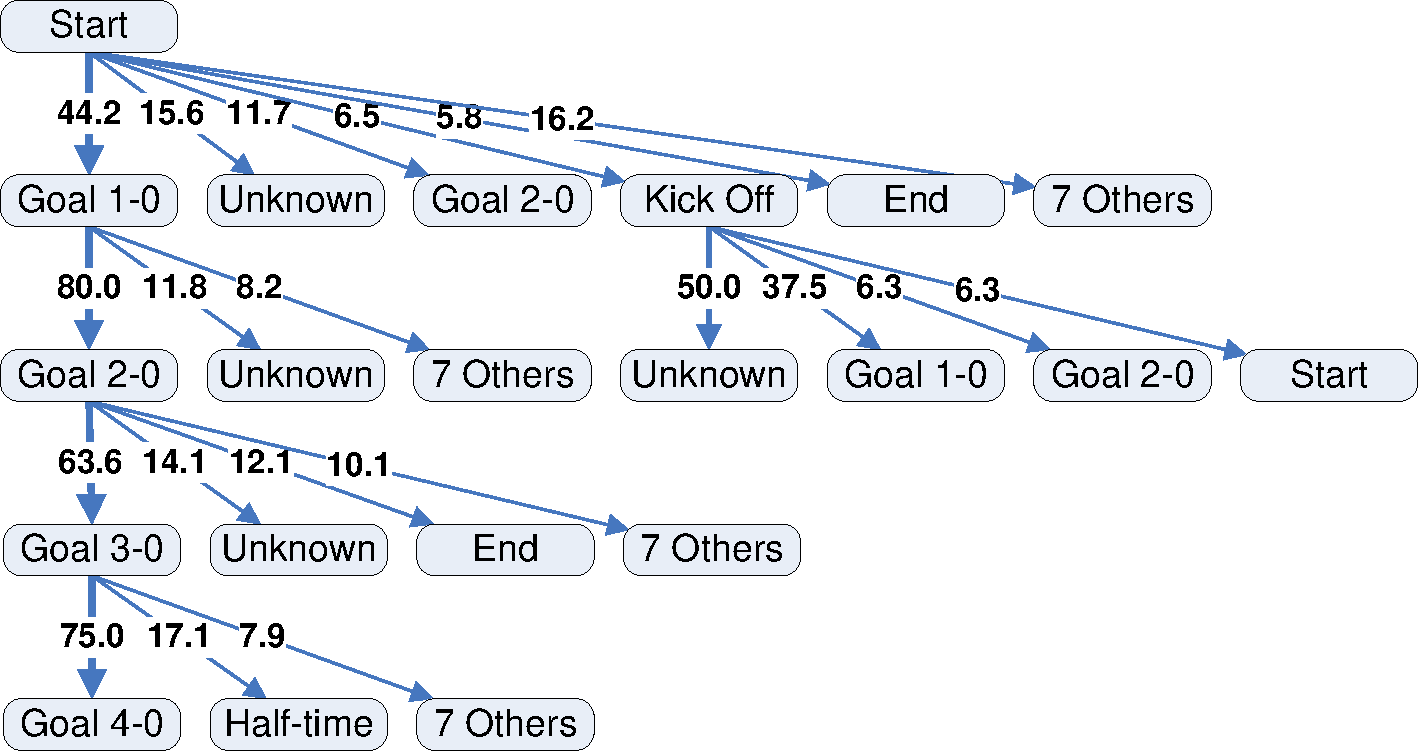
\includegraphics[width=0.50\columnwidth]{./diagrams/sequence}
    \caption{Sequence diagram for Argentina vs. Serbia and Montenegro depicted as a tree}
    \label{fig:sequences}
\end{figure}

\begin{figure}[t]
    %plotted with PlotSequence()
    \centering
    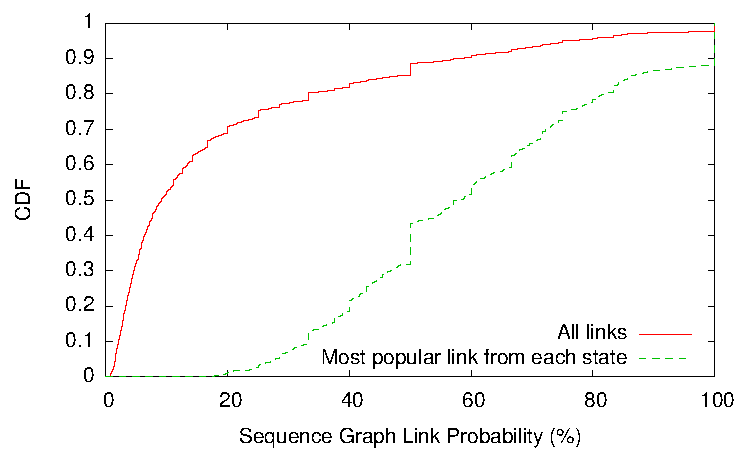
\includegraphics[width=0.50\columnwidth]{./graphs/all_sequence_normal_cdf}
    \caption{CDF of link probabilities for all videos}
    \label{fig:all_sequence}
\end{figure}

The traces were analysed to study the extent to which users' actions could be predicted. Since jumps to bookmarks made up a relatively large percentage of all requests, we limit this prediction to which bookmark will be visited next.
If a system could predict which bookmark would be requested next by a user, then it could pro-actively respond in order to optimise content delivery. For example, based on the next predicted bookmark, the relevant segments could be pushed out by a server with spare capacity, or pre-fetched by a client.

% 200seconds is longer than 96% of all interseek times
We call the order that bookmarks are viewed by a single user a {\em sequence} of bookmarks. Every user's sequence can be aggregated together to form a directed graph. Each node in the graph represents a bookmark with links between them representing the probability of seeking to that bookmark next. \autoref{fig:sequences} shows a section of one of these directed graphs depicted as a tree for clarity. The ``Start'' node represents the beginning of the video, and the ``End'' node represents the completion of a session. There is also an ``Unknown'' node which signifies when a seek to another bookmark has not been made within 200 seconds of visiting the previous bookmark (the observed upper bound for bookmarked events' length). For clarity, links with low probabilities have also been aggregated to form a ``$N$ Others'' node, where $N$ is the number of aggregated links.

It is clear from the figure that there are multiple choices to visit from each node, although there is generally one link that is significantly more likely to be chosen. For example, the probability of viewing bookmark ``Goal 2-0'' immediately after ``Goal 1-0'' is 80\%. We can also see that following the ``Kick Off'' bookmark 50\% of users did not visit another bookmark within 200 seconds and instead continue to watch, this could indicate that this subset of users were interested in watching the full game instead of just the highlights. An interesting observation for caching is the occurrence of self-loops. 6\% of links were between the same two bookmarks, which made up 6.5\% of all requests.

To understand how many bookmark-to-bookmark links are predictable, \autoref{fig:all_sequence} shows a CDF of probabilities for all links for all videos, as well as probabilities for just the most popular link from each bookmark. From this figure we can conclude that 10\% of all links have more than a 58\% chance of being followed.
Looking at just the most popular link from each bookmark we observe that over half of the bookmarks have an outgoing link with a probability over 50\%; an encouraging result for user predictability.

In this analysis we assumed that all users will visit the bookmark in similar order, however in a large heterogeneous environment this may not be true. Different sub-groups may wish to view a different set of events possibly in a different order to other sub-groups. Across our videos we did try and identify if there were groups of individuals that behaved differently to the majority, however none were found. This could possibly be due to our genre of media, with all sports fans wishing to see the same events, in the natural sequential order.

%Fig.~\ref{fig:all_sequence} shows that around the top 20\% of bookmark sequence pairs were followed by more than 50\% of users. This means that there is a high chance of predicting these bookmark sequences. Note that these bookmarks also consist of the 20\% most popular bookmarks. However, the figure also shows that it is generally difficult to predict the actions of a user if all actions are considered. This is because of the wider range of interactivity options a user has when VCR functionality is also considered.

%The exact parameters are of little importance, however the type of distribution used implies the impact on the system.

%Observe that
%the {\em log-normal} distribution emerges as the best model for most
%of the observed features in our experiment, except for object
%popularity and arrival rates, which are best modelled by {\em Normal
%} and {\em Weibull} distributions respectively. This is unsurprising
%because log-normal distributions are commonly known to model various
%properties in computing systems. Weibull and, as noted earlier,
%log-normal distributions both closely relate to power-law or
%heavy-tailed distributions~\cite{geor06}.

\begin{figure}[t]
    \centering

    % Plotted with PlotBookmarkWaitsMerge

    \subfloat[][Argentina vs. Serbia and Montenegro] {
        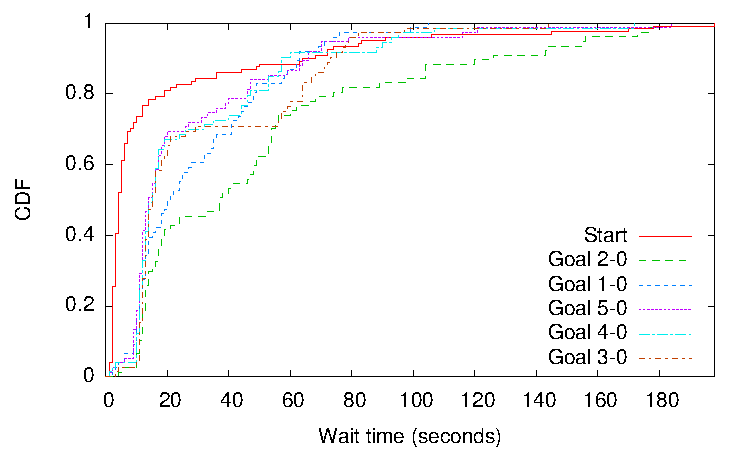
\includegraphics[width=0.5\columnwidth]{./graphs/arg-scg_all_waitjumps}
        \label{fig:waitjumps-a}
    }
    \subfloat[][Eurovision] {
        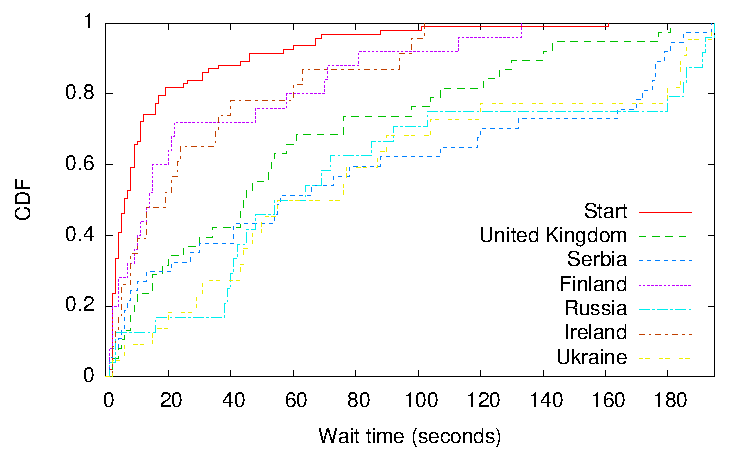
\includegraphics[width=0.5\columnwidth]{./graphs/eurovision_all_waitjumps}
        \label{fig:waitjumps-b}
    }

    \caption{CDFs of wait times}
    \label{fig:waitjumps}
\end{figure}

\section{Hotspot Length}
\label{sect:hotspot_length}

Jumps to bookmarks comprised roughly 20\% of all requests with an additional 32\% of seeks being within 60 seconds of a bookmark. Bookmarks form the majority of requests within the content, and represent the beginning of a popular segment of video which we call a \emph{hotspot}. The beginning of a hotspot is generally known (\emph{i.e.}, the bookmark point), but the end is not. Knowing the length of the hotspot can be useful for numerous tasks such as caching and pre-fetching. We therefore define \emph{wait time} as the time elapsed between a user following a bookmark and seeking.

\autoref{fig:waitjumps-a} \& \autoref{fig:waitjumps-b} show a CDF of wait times for each bookmark in the \emph{arg-scg} and \emph{eurovision} videos. It can be seen that in the football match the wait times follow a similar distribution, with the majority of users waiting less than 40 seconds (this, for example, could corresponds to the length of a run up to a goal). The \emph{eurovision} results are more varied with average wait times being much longer. This is due to the typical song in the Eurovision Song Contest being 180 seconds in length.  Finally, there is a ``Start'' bookmark listed in both figures: this is the entry point into both videos, and does not correspond to any event.

To better understand the wait times, distributions were fitted. In the general aggregated case a Weibull model fits best with parameters $\lambda=24.594$ and $k=0.7034$. For individual bookmarks log-normal and Weibull models proved best in the majority of cases.
%This result is similar to the inter-seek times in Section~\ref{sect:interseek}.
With these models the upper bound of a hotspots' lengths can be extrapolated by using, for example, the 95\sth percentile.

%'Log-Normal'    'R_SQUARE ='    [0.98463]    'TEST ='    [0.1127]    'MU ='    [2.6361]    'SIGMA ='    [1.388]
%'Weibull'    'R_SQUARE ='    [0.99545]    'TEST ='    [0.033063]    'l ='    [24.594]    'k ='    [0.7034]
%'Zipf'    'R_SQUARE ='    [0.93259]    'TEST ='    [0.34879]    's ='    [1.018]

\section{User Behaviour Models}

\begin{table}[tbp]
    \centering{\small
    \begin{tabular}{|rcc|}
      \hline
\setrowcolor{TableRowHead}
      Metric & Distribution & R-square \\
      \hline
\setrowcolor{TableRowA}
      Object Popularity  & Normal ( $\mu=60.129$ , $\sigma=32.111$ )     & 0.97996 \\
\setrowcolor{TableRowB}
      Segment Popularity & Log-normal ( $\mu=0.551$ , $\sigma=1.32$ )   & 0.98084 \\
\setrowcolor{TableRowB}
                         & Weibull    ( $\lambda=2.887$ , $k=0.69527$ ) & 0.98284 \\
\setrowcolor{TableRowA}
      Session Length     & Log-normal ( $\mu=4.73$, $\sigma=1.90$ )     & 0.99779  \\
\setrowcolor{TableRowA}
                         & Weibull    ( $\lambda=233.17$, $k=0.51125$ ) & 0.98666 \\
\setrowcolor{TableRowB}
      Inter-seek times   & Log-normal ( $\mu=1.2886$, $\sigma=2.318$ )  & 0.99644 \\
\setrowcolor{TableRowB}
                         & Weibull    ( $\lambda=7.5243$, $k=0.35646$ ) & 0.99353 \\
\setrowcolor{TableRowA}
      Seek Distance (forward)      & Log-normal ( $\mu = 7.2668$, $\sigma = 1.2194$ )  & 0.99567 \\
      \setrowcolor{TableRowB}
      Seek Distance (backward)     & Log-normal ( $\mu = 7.195$, $\sigma = 1.3132$ )   & 0.99083 \\
\setrowcolor{TableRowA}
      Hotspot Length    & Log-normal ( $\mu=2.6361$, $\sigma=1.388$ )  & 0.98463 \\
\setrowcolor{TableRowA}
                         & Weibull    ( $\lambda=24.594$ , $k=0.7034$ ) & 0.99545 \\
\setrowcolor{TableRowB}
      Bookmark Longevity & Weibull    ( $\lambda=3.1004$ , $k=0.61592$ ) & 0.99796 \\
    \hline
    \end{tabular}
    }
    \caption{A summary of metrics with their corresponding distributions}
    \label{tab:models}
\end{table}

Model fitting is important for understanding the different properties of the system, and aids in simulation creation and algorithmic design. Various models have been discussed for the different parameters of the system. In all cases many models (\emph{e.g.}, normal, log-normal, exponential, Weibull, Pareto, Poisson, Zipf) were fitted to the data with varying success. Generally, more than one distribution fitted well. This subsection will summarise the analytical models found for each parameter.

\autoref{tab:models} gives an overview of the best matching models for each metric discussed previously, with their corresponding \emph{R-square} values. Of particular importance are the types of distribution which can have a significant impact on the system. For example, the Weibull and log-normal models are both long-tailed, and systems may have to anticipate the skewed distribution to cope effectively.

%\begin{table}[tb]
%    \centering\scriptsize
%
%    \begin{tabular}{|ccccccccc|}
%      \hline
%\setrowcolor{TableRowHead}
%      Metric & Max Models & Log-normal & Weibull & Pareto & Normal & Exponential & Zipf & No fit\\
%      \hline
%\setrowcolor{TableRowA}
%      Segment Popularity & 84 (from 88 videos) & 61  & 65  & 12 & 58 & 42 & 13 & 17\\
%\setrowcolor{TableRowB}
%      Session Length     & 81 (from 88 videos) & 75  & 72  & 0  & 5  & 31 & 4  & 0\\
%\setrowcolor{TableRowA}
%      Inter-seek times   & 87 (from 88 videos) & 83  & 83  & 54 & 1  &  3 & 55 & 3\\
%\setrowcolor{TableRowB}
%      Hotspot Length    & 203 (from 695 bookmarks) & 165 & 135 & 91 & 5  & 48 & 53 & 22 \\
%      \hline
%    \end{tabular}
%    \caption{Metrics for individual videos and their corresponding distributions}
%    \label{tab:models_all}
%\end{table}
%
%The models shown so far are from aggregated results across all the videos. Instead, it may be interesting to model the different metrics of each particular video. However due to the diversity in models and parameters it is not possible to show each model, so instead \autoref{tab:models_all} summaries which models fit with a \emph{R-square} value greater than 95\%. The ``max models'' column represents the number of datasets that are of sufficient size to have models fitted. For example, there are 695 bookmarks, yet only 203 had enough data to be fitted to a hotspot length, and of these, 165 fitted well to a Log-normal model, 135 to a Weibull models, \emph{etc}.

\section{Summary}

%In this section we have shown:
%    When presented with bookmarks users are highly influences by them
%    This causes the popularity of seconds to be heavy-tailed
%    Session times are very short compared to media
%    A sequence of bookmarks can be predicted
%
%    Can we make sure bookmarks help the system as much as possible?
%    Can we predict which bookmark is next?

Our results have shown that the interactivity options available to users highly influence their behaviour. In particular, it was found that the novel interactive feature of \emph{bookmarking} played a pivotal role, leading to access patterns quite dissimilar from previous related studies that looked at VCR-like interactivity alone.
The combination of our content type and the addition of bookmarks led to users accessing content in relatively short segments sparsely distributed throughout the length of the videos. Segment popularity is skewed with the most popular segments clearly around the bookmarks, forming hotspots. From both a user and a content distribution network's perspective, this can be viewed as advantageous; users can reach interesting content more quickly through the bookmarks, and the increased locality of interest means CDNs can respond more effectively by, for example, prioritising hotspot replication.

Content placement is an important and difficult problem for CDNs. The CDN has to decide where within the network to replicate or cache content. Typically the content is placed near to the users, and replicated as a whole. However, as we have seen, not all segments within a piece of content are equal and a CDN can leverage this information to replicate certain segments more than others. This is especially useful when popularity nearly always concentrates around bookmarks, allowing the relevant segments to be replicated throughout the network before user demand increases.

A CDN could be designed to handle high levels of user interactivity, with relatively short sessions and inter-seek times. Our results have shown that hotspots following bookmarks were orders of magnitude shorter than the video containing them. Furthermore, it encourages the use of an agile delivery mechanism that allows distribution of small sparsely distributed segments quickly and efficiently.

We have also shown that users view the bookmarks in a similar order, giving them a degree of predictability. This could allow a CDN to exploit pre-fetching techniques to improve the user's experience. For example, if the CDN could predict the next segment the user will watch, then this could be pre-fetched into the user's playback buffer and when the user seeks to that segment there will be no delay caused by seek latency and buffering.

The use of bookmarks depends on them being well positioned and of interest to the user. We noted in the first experiment that 40\% of bookmarks had at least one user seek before the bookmark, with 30.7\% of these seeks occurring within 5 seconds of jumping to the bookmark. This perhaps represents users who were almost immediately dissatisfied with the bookmark's location. We noted this happened consistently for roughly 6\% of the total bookmarks. Upon further inspection, it appeared the bookmarks were inadvertently misplaced. This led to users performing additional seeks to find the correct location, thus placing extra load on the servers.

% CHECKME
Throughout the experiment different genres of videos were available to the users, namely sporting and musical videos. Only the analysis of the ``Argentina vs. Serbia and Montenegro'' football match and the ``Eurovision song contest'' were shown in this chapter, however other sporting events were available on the site such as Formula~1 racing, International Cricket, and other miscellaneous recordings of music channels. Similar patterns were observed for each video, however, semantics of the content did have some impact of how the users consumed the data.

All videos exhibited similar patterns, for example, popularity was generally centered around the bookmarked segments, and that the viewing duration was far shorter than the full length of the video. However, minor differences were found, for example, the music channels had greater variance in the popularity of each bookmark (which were placed at the beginning of individual music videos). This can easily be attributed to users only being interested in particular artists or videos, whereas viewers of sporting events would be interested in every highlight (and therefore every bookmark). Similar differences were found in the inter-seek times, session times, and hotspot lengths, as the semantics of the content would determine how long particular hotspots were. However, metrics such as the number of interactions, or bookmark longevity stayed the same, as these did not appear to be directly impacted by the content.

In the following chapter, we explore and study the implications of a few techniques designed to exploit some of the properties suggested from our analysis. The first addresses the dynamic re-positioning of bookmarks in response to user behaviour. The second concerns predictive pre-fetching of popular segments to enhance the efficiency of delivery of highly interactive content. The last technique is an evaluation of how well existing delivery mechanisms behaviour when delivering interactive media, and how this can be improved with an hybrid approach.
